
In \acrfull{MBT}, test cases are selected automatically from a partial representation of expected behaviour of the \acrfull{SUT} (\ie the model). For most systems, it is intractable to select all the possible test cases from the model. The test engineer relies on selection algorithms that maximize a given criterion, a metric one the adequacy of a test suite \cite{Mathur2008}. In this chapter, we define the notion of \emph{abstract test case} (in Section \ref{sec:coverage:asbtracttestcase}), a test case selected from a \acrfull{FTS}, a mathematical structure to compactly represent the behaviour of a SPL (see Definition \ref{def:fts}). Based on this definition, we describe  three families of criteria: 
\begin{enumerate}
\item \emph{structural selection criteria} (in Section \ref{sec:coverage:structuralcrit}), adapted from the classical \glspl{labelled transition system} to \glspl{FTS} \cite{Devroey2014e};
\item \emph{dissimilarity selection criteria} (in Section \ref{sec:coverage:dissimilaritycrit}), which aims at selecting abstract test cases as dissimilar as possible, both in terms of behaviour and in terms of products covered by the test cases \cite{Devroey2016};
\item and \emph{usage selection criteria} (in Section \ref{sec:coverage:usagecrit}), which selects abstract test cases based on the previous usage of the \gls{SPL} \cite{Devroey2015a,Devroey2014}.
\end{enumerate}
For each criterion, we give its definition, an abstract test case selection algorithm, and prioritisation methods to prioritize the products of the \gls{SPL} required to execute the selected abstract test cases.


%%%%%%%%%%%%%%%%%%%%%%%%%%%%%%%%%%%%%%%%%
\section{Abstract test case over an FTS}
%%%%%%%%%%%%%%%%%%%%%%%%%%%%%%%%%%%%%%%%%

\label{sec:coverage:asbtracttestcase}

In a \gls{MBT} approach, test cases are automatically selected from a model of the system under test. This derivation is done in several steps: first, \emph{\glspl{abstract test case}} are selected from the model, an FTS in our case, using a given criterion; those abstract test cases are then refined, using additional information in order to be executable by the \gls{SUT}. This section, and the remainder of this chapter cover the first step: abstract test case selection. Chapter \ref{chap:concretization} covers the second step: abstract test case concretization.

First, let us define the notion of abstract test case for FTSs. We define an abstract test case over an FTS as a sequence of \emph{actions} from this FTS, such that there exists a sequence of \emph{transitions} in this FTS with the given actions.
%
\begin{definition}[\Gls{abstract test case}] \label{def:atc}
Let $\fts = (S,$ $\Act,$ $\trans,$ $i,$ $d,$ $\gamma)$ be an FTS. An abstract test case $t$ is a finite sequence $(\alpha_1,\ldots, \alpha_n)$, where $\alpha_1,\ldots, \alpha_n \in Act$ and there exists a sequence of transitions in $\trans$ such that 
$$i \xrightarrow{\alpha_1} s_k \xrightarrow{\alpha_2} \ldots \xrightarrow{\alpha_n} s_l $$
\end{definition} 
%

For instance, an abstract test case for the \gls{soda vending machine} SPL described in Section \ref{sec:casestudy:svm} may be \textit{(pay, change, soda, serve\-Soda)}. This abstract test case is a sequence of actions in the FTS (see Figure \ref{fig:svmfts}) representing a behaviour of this SPL.

%--------------------------------------------------------
\subsection{Positive and negative abstract test cases}
%--------------------------------------------------------

We distinguish two kinds of test cases: \emph{positive test cases} trigger a desired/expected behaviour of the system under test; and \emph{negative test cases} trigger an undesired behaviour of the system under test \cite{Jobstl2014,Utting2007}. In our case, a \gls{positive abstract test case} is defined as a sequence of actions executable by the $\fts$, while a \gls{negative abstract test case} is a sequence of actions not executable by the $\fts$. Once concretized, negative abstract test cases typically represent sequences of actions that every product of the product line should forbid. 

In a LTS ($\lts$), an abstract test case $t=(\alpha_1,\ldots, \alpha_n)$ is executable, denoted $\lts \overset{t}{\Longrightarrow}$, if there exists a sequence of transitions starting from the initial state and labelled with $\alpha_1,\ldots, \alpha_n$~\cite{Tretmans2008,Tretmans2011}. For an FTS ($\fts$), to be executable, the sequence of transition must moreover have compatible feature expressions. In other words, a sequence of actions is executable by $\fts$ if there exists at least one product ($p$) which, when $\fts$ is projected onto $p$ (denoted $\fts_{\mid p}$), is able to execute it:
%
$$ 
\left( \fts \overset{\alpha_1,\ldots, \alpha_n}{\Longrightarrow} \right) 
\Leftrightarrow 
\left(\exists p \in \Sem{d} : \fts_{\mid p} \overset{\alpha_1,\ldots, \alpha_n}{\Longrightarrow} \right) 
$$
%

\paragraph{Example:} 
%---------------------

For instance, the abstract test case \textit{(pay, change, soda, serve\-Soda, take)} is not executable on the soda vending machine FTS since it mixes both vending machines that offers free drinks and vending machines that do not. Practically, this can be detected in the FTS (and the FM) by detecting incompatible feature expressions on the transitions: $\neg f$ on transitions $s_1 \xrightarrow{pay/\neg f} s_2$ and $s_2 \xrightarrow{change/\neg f} s_3$, and $f$ on transition $s_7 \xrightarrow{take/f} s_1$.

In testing, unlike model checking~\cite{Baier2008}, we only consider finite sequences of actions. Since FTSs (as LTSs) do not have final/accepting state \textit{per se}, in order to decide if a sequence of actions represents a desired behaviour of the system, we chose to consider the initial state of an FTS as a final state. Positive abstract test cases have to end their execution in the initial state (\eg state $s_1$ in the soda vending machine FTS).

\begin{definition}[\Gls{positive abstract test case}] \label{def:postc}
Let $fts=(S,$ $Act,$ $trans,$ $i,$ $d,$ $\gamma)$ be an FTS. A positive abstract test case $t=(\alpha_1,\ldots, \alpha_n)$, where $\alpha_1,\ldots, \alpha_n \in Act$, is a finite sequence of actions such as there is at least one product from $d$ able to execute $t$, and this execution ends in the initial state:
$$\exists p \in \Sem{d} : fts_{\mid p} \overset{t}{\Rightarrow} i$$
\end{definition}

\begin{definition}[\Gls{negative abstract test case}] \label{def:negtc}
Let $fts=(S,$ $Act,$ $trans,$ $i,$ $d,$ $\gamma)$ be an FTS. A negative abstract test case $t=(\alpha_1,\ldots, \alpha_n)$, where $\alpha_1,\ldots, \alpha_n \in Act$, is a finite sequence of actions such as for every product from $d$, the product is not able to execute $t$ or this execution does not end in the initial state:
$$\forall p \in \Sem{d} : fts_{\mid p} \overset{t}{\nRightarrow} i$$
\end{definition} 

When derived from the soda vending machine FTS, a positive abstract test case has to start from $s_1$ and end in $s_1$ and only fire transitions with compatible feature expressions. For instance, abstract test case \textit{(free, soda, serve\-Soda, take)} is a positive abstract test case, while \textit{(free, soda, serve\-Soda, open, take, close)} and \textit{(free, soda, serve\-Soda)} are negative abstract test cases (the first one fires transitions with incompatible feature expressions and the second one does not end in the initial state when it is executed on the FTS).

In the remainder, we mainly focus on positive abstract test cases and simply write \emph{test case}. A \emph{test suite}, defined for a \gls{SUT}, is a set of test cases.


%--------------------------------------------------------
\subsection{Test suite product selection}
%--------------------------------------------------------

When abstract test cases are concretized, the result (\ie concrete test cases, represented as a sequence of operations on the system) has to be executed on one or more products of the SPL. The set of products able to execute a test case may be calculated from the FTS (and the FM). It corresponds to all the products (\ie set of features) of the FM that satisfy all the feature expressions associated to the transitions fired by the abstract test case when it is executed on the FTS:
%
\begin{definition}[Test case product selection]
Given an FTS $fts = (S,$ $\Act,$ $\trans,$ $i,$ $d,$ $\gamma) $ and a positive abstract test case $t = (\alpha_1 ,$ $ \ldots ,$ $ \alpha_n)$ with $(\alpha_1 $ $, \ldots $ $, \alpha_n)$ $ \in \Act$, the set of products able to execute $t$ is defined as:
%
$$ \wProd(\fts, t) = \{ p \in \Sem{d} \mid fts_{\mid p} \overset{t}{\Longrightarrow} i\}
$$
%
\end{definition}
It corresponds to all the products able to execute the sequence of actions in $t$. 
%
From a practical point of view, the set of products contains all the products satisfying the conjunction of the feature expressions $\gamma (s_k \overset{\alpha_i}{\longrightarrow} s_{k+1}) $ on the path(s) of $t$ and the FM~$d$. When $d$ is boolean, it may be transformed to a boolean formula in \gls{CNF} where features become variables~\cite{Czarnecki2007}. The existence of a product for a test case is equivalent to the satisfiability of the following formula, that can be checked by a SAT solver:
%
$$\bigvee_{\mathit{pt} \in \mathit{paths}} \left(\bigwedge_{i=1}^{n_{\mathit{pt}}} \left( \gamma (s_k \overset{\alpha_i}{\longrightarrow} s_{l}) \right) \right) \wedge \mathit{CNF}(d)$$
%
For instance, the set of products for the test case \textit{(free, soda, serve\-Soda, take)}, derived from the vending machine FTS, contains all the products of the SPL that offer free soda.
%
Similarly, for a test suite, we have:
%
\begin{definition}[Test suite product selection]
Given an FTS $\fts = (S,$ $\Act,$ $\trans,$ $i,$ $d,$ $\gamma) $ and a test suite $s=\{t_1 , \ldots , t_n \}$, where $t_1, \ldots, t_n$ are positive abstract test cases, the set of products able to execute the test suite:
$$\wProd(\fts, s) = \bigcup_{t_i \in s} \wProd(fts, t_i)$$
\end{definition}
If we have a test suite ($s$) with two test cases \textit{(free, soda, serve\-Soda, take)} and \textit{(free, tea, serve\-Tea, take)}, the set of products contains all the products of the SPL that offers free soda or free tea.

We will consider that for a given test suite ($s$), a set of products ($M$) is adequate, if $M$ contains enough products to execute the test cases in $s$:
\begin{definition}[$s$-adequate set of products]
Let $\fts$ be an FTS and $s = \{t_1 , \ldots , t_n \}$ be an abstract test suite where $t_1, \ldots, t_n$ are positive abstract test cases. The set of products $M$ is $s$-adequate, denoted $M\overset{s}{\Longrightarrow}$, if each test case in $s$ may be executed by at least one product in $M$:
$$\forall t \in s: \exists p \in M, \fts_{\mid p} \overset{t}{\Longrightarrow} i $$
\end{definition}

Since one of the main concern in SPL testing is to reduce the number of products needed to execute the test, we also define the selection of the minimal $s$-adequate set of products required to execute a test suite:
%
\begin{definition}[P-Minimal test suite product selection]
Let $\fts$ be an FTS  and $s = \{t_1 , \ldots , t_n \}$ be an abstract test suite where $t_1, \ldots, t_n$ are positive abstract test cases. A minimal $s$-adequate set of products needed to execute the test suite, denoted $\wMprod(\fts,$ $s)$ $= M$, is a subset of $\wProd(\fts, s)$ such that $M$ is $s$-adequate and there is no subset of $M$ that is $s$-adequate: 
$$ \left( M\overset{s}{\Longrightarrow} \right) \wedge \left( \forall M' \subset M, \left( M'\overset{s}{\not\Longrightarrow} \right) \right) $$
\end{definition}

\paragraph{Example (continued):} 
%---------------------------------

There are two products able to execute all the test cases in the test suite $s$: one that allows to cancel purchase and one that doesn't. The p-Minimal set of products for $s$ is a set with only one of those two products. The decision of the products to include (or not) should be taken by the test engineer, depending for instance on the cost linked to the derivation of each product.


%%%%%%%%%%%%%%%%%%%%%%%%%%%%%%%%%%%%%%%
\section{Structural selection criteria}
%%%%%%%%%%%%%%%%%%%%%%%%%%%%%%%%%%%%%%%

\label{sec:coverage:structuralcrit}

In order to efficiently select test cases, the test engineer has to provide \emph{selection criteria}~\cite{Mathur2008,Utting2007}.
%
We redefine hereafter classical structural coverage selection criteria for \emph{connected} FTSs as a function, returning for a given FTS and a test suite, a value between 0 and 1 specifying the coverage degree of the executable abstract test suite over the FTS: $0$ meaning no coverage and $1$ the maximal coverage. 

\begin{definition}[\Gls{coverage criterion}]
A coverage criterion is a function $cov$ that associates an FTS and a test suite over this FTS to a real value in $[0,1]$.
\end{definition}

Classical structural coverage criteria are defined as follow, we illustrate each coverage criteria with test suites satisfying the criteria for the \gls{soda vending machine} FTS defined in figure \ref{fig:svmfts}:

\begin{definition}[State/All-states coverage]
The state coverage criterion is related to the ratio between the states visited by the test cases pertaining to the test suite and all the states of the FTS. When the value of the function equals to $1$, the test suite satisfies the \emph{all-states coverage}.    
\end{definition}

\paragraph{Example (continued):} 
%---------------------------------

The all-states selection criterion is the weakest structural selection criterion \cite{Utting2007}, it specifies that when executing the test suite, each state has to be visited at least once. On the soda vending machine, an all-states covering test suite may be: 
\begin{quote}
\textit{\{ (pay, change, soda, serveSoda, open, take, close); \\
(free, tea, serveTea, take);\\
(free, cancel, return) \}}
\end{quote}

\begin{definition}[Action/All-actions coverage]
The action coverage criterion is related to the ratio between the actions triggered by the test cases pertaining to the test suite and all the actions of the FTS defined. When the value of the function equals $1$, the test suite satisfies \emph{all-actions coverage}.    
\end{definition}
%
In this case, a satisfying test suite for a coverage of $1$ on the soda vending machine may be the same as the one defined for the all-states coverage.  

\begin{definition}[Transition/All-transitions coverage]
Transition coverage is  related to the ratio between transitions covered when running test cases on the FTS and the total number of transitions of the FTS. When this ratio equals to $1$, then the test suite satisfies \emph{all-transitions} coverage.    
\end{definition}
%
The all-transitions coverage specifies that, ideally, each transition is fired at least once when executing the abstract test suite on the FTS. Again, the test suite defined using the the all-states coverage criteria satisfies the all-transitions coverage.  

\begin{definition}[Transition-pair/All-transition-pairs coverage]
The tran\-si\-tion-pairs coverage considers adjacent transitions successively entering and leaving a given state. When the coverage function reaches the value of $1$, then the test suite covers \emph{all-transition-pairs}. 
\end{definition}

\paragraph{Example (continued):} 
%---------------------------------

The all-transition-pairs coverage specifies that for each state, each couple of entering/leaving transitions has to be fired at least once. On the soda vending machine, a test suite that covers all-transitions-pairs may be:
%
\begin{quote}
\textit{ \{ (pay, change, soda, serveSoda, open, take, close); \\
(pay, change, cancel, return);\\
(pay, change, tea, serveTea, open, take, close); \\
(free, soda, serveSoda, take);\\
(free, tea, serveTea, take); \\
(free, cancel, return) \}}
\end{quote}

\begin{definition}[Path/All-paths coverage]
Path coverage takes into account simple executable paths (\ie paths that does not fire the same transition twice), that is sequences of transitions starting from and ending in the initial state. If the coverage function value computing the ratio between the number of  simple executable paths covered by the test cases and total number of simple executable paths in the FTS is $1$, \emph{all-paths} coverage has been reached.  
\end{definition}
%
The all-path coverage specifies that each simple executable path in the FTS should be followed at least once when executing the test suite. On the soda vending machine, it gives a test suite equal to the one defined for all-transitions-pair coverage.


%------------------------------------------------
\subsection{All-states selection algorithm}
%------------------------------------------------

\label{subsec:allstatesselection}

We present hereafter a (simple) algorithm to select a test suite satisfying the all-states coverage criteria. This algorithm builds abstract test cases iteratively, using a heuristic based on an accessibility matrix for the FTS. The idea is to start from the initial state with an empty abstract test case and a $true$ feature expression. At each iteration, the algorithm branches out the current partial abstract test case into multiple partial abstract test cases, one per outgoing transition. For each transition, if the feature expression of the transition is compatible, the corresponding action is added to one of the partial abstract test cases. The algorithm then selects the partial abstract test case with the highest score: \ie the one where the target state of the selected transition may lead to the highest number of states that has not yet been visited by a previously computed abstract test case. The target state becomes then the new current state for the next iteration, and the feature expression associated to the transition is conjoined with the current feature expression.

We present hereafter three algorithms involved in the computation of a all-states covering test suite: the computation of the \emph{accessibility matrix} for a FTS using a variant of the Warshall algorithm \cite{Rosen2011}, the \emph{heuristic} which computes for a given state its score, and finally the \emph{selection algorithm} which computes the test suite satisfying the all-states coverage criterion. 

\paragraph{Accessibility matrix computation:}
%--------------------------------------------

The accessibility matrix $A$ gives for two states $(s_1, s_2)$ the products able to execute a non-empty paths from $s_1$ to $s_2$. This matrix corresponds to the transitive closure of the \gls{FTS} and is computed using the Warshall algorithm \cite{Rosen2011}. 
Contrary to an accessibility matrix computed for a classical LTS, the entry for $s_1$ and $s_2$ (noted $A[1,2]$) is not $true$ or $false$ (\ie there exists a path from $s_1$ to $s_2$ or not), but rather the products for which there exists a path from $s_1$ to $s_2$.

In our implementation of the algorithm, as for in ProVeLines \cite{Cordy2013}, the products able to execute a transition $tr$ (noted $\gamma\ tr$) are represented using feature expressions (\ie boolean expressions over features). An entry of the accessibility matrix $A$ is a feature expression. \Eg for the soda vending machine in Figure \ref{fig:svmfts}, the simplified entry $A[1,4]$ is $(\neg f \vee f) \wedge c$, states that there exists a path in the FTS from $s_1$ to $s_4$ for all the products of the SPL having the $cancel$ feature and having or not $free$ drinks.

\begin{algorithm}
 \KwIn{$\fts = (S,Act,\mathit{trans},i,d,\gamma)$: a connected FTS}
 \KwOut{$A$: an accessibility matrix}
 \Begin{
	 $\forall s_i, s_j \in S: A[i,j] = \bigvee_{t = (s_i, \alpha, s_j) \in trans} \gamma t \, $\; \nllabel{algo:warshall:line:init}
	 \For{$k \in [1, \#S]$}{
	 	\For{$i \in [1, \#S]$}{
		 	\For{$j \in [1, \#S]$}{
				$A[i,j] = A[i,j] \vee (A[i,k] \wedge A[k,j])$\; \nllabel{algo:warshall:line:allintermediatepath}
	  	}	}
	 }
	 \Return $A$\;
 }
 \caption{Warshall algorithm computing the accessibility matrix of an FTS}
 \label{algo:warshall}
\end{algorithm}

Algorithm \ref{algo:warshall} presents the adaptation of the Warshall algorithm for FTSs. The output of the algorithm is the accessibility matrix $A$ for the given FTS. First $A$ is initialised with the feature expressions conditioning the transition from one state to another (line \ref{algo:warshall:line:init}). In the next steps, the matrix is updated by computing all the possible intermediate paths for each pair of states (line \ref{algo:warshall:line:allintermediatepath}). 

\paragraph{Score computation:}
%------------------------------

Once we have the accessibility matrix, we use a branch and bound algorithm which explores the FTS according to our heuristic. We choose a simple heuristic: it computes a score equal for a given state to the number of states not yet covered by current test suite and accessible from this state. 

\begin{algorithm}
 \KwIn{$A$: an accessibility matrix; \\
 $k$: the index (in $A$) of the current state;\\
 $e$: a feature expression;\\
 $d$: the feature model;\\
 $\mathit{toVisit}$: the states not yet covered;}
 \KwOut{$\mathit{score}$: the score associated to $s_k$}
 \Begin{
	 $score = 0$\;
	 \For{$j \in [1; \#S]$ \nllabel{algo:allstatesheuristic:line:loop} }{
	 	\If{$s_j \in \mathit{toVisit} \wedge \mathit{SAT}(A[k,j] \wedge \CNF(d) \wedge e)$ \nllabel{algo:allstatesheuristic:line:verif}}{
	 		 $\mathit{score} = \mathit{score} + 1$\; \nllabel{algo:allstatesheuristic:line:increment}
	 	}
	 }
 }
 \Return $score$\;
 \caption{Partial abstract test case score computation}
 \label{algo:allstatesheuristic}
\end{algorithm}

Algorithm \ref{algo:allstatesheuristic} presents the score computation for a given accessibility matrix $A$ and a state $s_k$.
This score is computed dynamically during the selection of an abstract test case by iterating over the $k$-th line of the accessibility matrix $A$ (line \ref{algo:allstatesheuristic:line:loop}). The score is incremented by $1$ for every cell corresponding to a not yet reached state (line \ref{algo:allstatesheuristic:line:increment}). Before the increment, we verify (at line \ref{algo:allstatesheuristic:line:verif}) that the feature expression is compatible with the feature model and the actual partial abstract test case feature expression $e$ (\ie there exist one product able to execute the partial abstract test case) using a SAT call and the \gls{CNF} representation of the feature model $d$.

\paragraph{All-states covering abstract test suite selection:}
%------------------------------------------------------------

\begin{algorithm}[t]
 \KwIn{$\fts=(S,\Act,\trans,i,d,\gamma)$: a connected FTS;\\
 $A$: the accessibility matrix of $\fts$;}
 \KwOut{$ts$: the selected test suite}
 \Begin{
	 \textit{toVisit = S} \; \nllabel{algo:allstatesselection:line:inittovisit}
	 \textit{candidates = }$\emptyset $\;
	 \ForEach{$tr = (i, \alpha, s_k) \in \trans$ \nllabel{algo:allstatesselection:line:candidatesinit}}{
	 	\textit{candidates = candidates} $\cup \left\lbrace \left((tr), \wScore(A, k, \gamma tr, \wToVisit) \right)  \right\rbrace$\;
	 }
	 \textit{testsuite =} $\emptyset $\; \nllabel{algo:allstatesselection:line:inittestsuite}
	 \While{\textit{toVisit} $\neq \emptyset$ \nllabel{algo:allstatesselection:line:mainloop}}{
	 	$c = (\wPath, \wScore) \in$ \textit{candidates} such as $\wScore$ is maximal in \textit{candidates}\; \nllabel{algo:allstatesselection:line:bestc}
	 	\textit{candidates = candidates }$\setminus \{c\}$\;
	 	\eIf{last state of $c.\wPath$ is $i$ \nllabel{algo:allstatesselection:line:initreached}}{
	 		\If{$c.\wPath$ contains states from $\wToVisit$}{
	 			add sequence of actions on $c.\wPath$ to \textit{testsuite}\; \nllabel{algo:allstatesselection:line:addtestsuite}
		 		remove states on $c.\wPath$ from $\wToVisit$\; \nllabel{algo:allstatesselection:line:removevisited}
	 		}
	  	}{
	  		\ForEach{transition $tr$ starting from last state of $c.\wPath$}{
	  			\textit{fexpr =} $\bigwedge_{tr_i \in c.\wPath} (\gamma tr_i) \wedge (\gamma tr) \wedge \CNF(d) $\;
	  			\If{\textit{SAT(fexpr)} \nllabel{algo:allstatesselection:line:ifsat}}{
	  				$c' = (c.path ++ tr, score(A, k, \mathit{fexpr}, \wToVisit))$\; \nllabel{algo:allstatesselection:line:newct}
			  		$candidates = candidates \cup \left\lbrace c' \right\rbrace$\; \nllabel{algo:allstatesselection:line:addcandidate}
			  	}
	  		}  		
	  	}
	 }
     \Return $testset$\;
 }
 \caption{All-states test suite selection}
 \label{algo:allstatesselection}
\end{algorithm}

The all-states test suite selection algorithm is described in Algorithm \ref{algo:allstatesselection}. This algorithm produces an abstract test suite that satisfies the all-states coverage criterion. 
First the states to visit set (\textit{toVisit}) is initialised to $S$ (line \ref{algo:allstatesselection:line:inittovisit}), all the states of the FTS. The candidates to consider (\textit{candidates}) are the paths with one transition going out from the initial state $i$ (line \ref{algo:allstatesselection:line:candidatesinit}). Each candidate is a couple with a path (\textit{path}) and a score computed using Algorithm \ref{algo:allstatesheuristic}. At this stage, the test suite (\textit{testsuite}) is empty (line \ref{algo:allstatesselection:line:inittestsuite}).

The main loop of the algorithm (line \ref{algo:allstatesselection:line:mainloop}) computes the abstract test cases and continues as long as states to visit in the FTS remain. In this loop, the best candidate $c$ (with the highest score) is picked (line \ref{algo:allstatesselection:line:bestc}) and removed from the list of candidates to consider. 

If the last state of this candidate is the initial sate $i$, we found an abstract test case (\ie the sequence of actions on the path) which is added to the test suite if the path contains states not yet visited (line \ref{algo:allstatesselection:line:addtestsuite}). 
The states of the path are removed from the states to visit (line \ref{algo:allstatesselection:line:removevisited}) and the algorithm picks the next candidate at the next iteration. 

If the last state reached by the abstract test case is not the initial state, the exploration continues and new candidates are computed. Each outgoing transitions of the last state of the path is added to a new candidate if there exists a product able to execute the new partial abstract test case (checked using a SAT call at line \ref{algo:allstatesselection:line:ifsat}) and for each one, a new score is computed (lines \ref{algo:allstatesselection:line:newct} and \ref{algo:allstatesselection:line:addcandidate}).

\paragraph{Simplification for large models:}
%-------------------------------------------

To scale to our largest models, a simplification has been implemented in the algorithm: we ignore the feature expressions and check the validity of a path (\ie the satisfiability of the feature expression) only before adding an abstract test case to the test suite (line \ref{algo:allstatesselection:line:addtestsuite}). Before adding the abstract test case to the test suite and removing the visited states from the $toVisit$ set, we perform a satisfiability call ($SAT$) on the conjunction of the feature model ($\mathit{CNF}(d)$) and the feature expression of the abstract test case (\textit{fexpr}). This simplification, implemented after our first run of the algorithm, reduces the number of SAT calls which are very costly, but might increase the number of invalid partial abstract test cases, depending on the feature models and the feature expressions in the FTS.

To avoid a explosion of the \textit{candidates} set, the paths and their scores may be represented using a tree structure, where states are nodes and transitions are branches between two nodes. A walk in the tree represents a path in the FTS.


%------------------------------------------------
\subsection{Test case and test suite minimality}
%------------------------------------------------

Usually, when performing test case selection, one wants to have a test suite as small as possible while ensuring the best coverage. Contrary to single systems where only the size of the test suite is taken into account, when performing SPL testing, we also have to consider the number of products needed to execute the test suite. We define the \emph{size} of a test suite as the number of transitions triggered by its test cases.

\begin{definition}[Test suite size]
The size of a test suite $s$ corresponds to the number of transitions triggered in a FTS $\fts$ when executing the test cases of $s$ on $\fts$, denoted 
$$\fts \overset{s}{\Longrightarrow}$$
\end{definition}
%
This allows to differentiate a test suite $s_1$ with test cases only triggering a minimal set of transitions to satisfy a coverage criterion from a test suite $s_2$ also satisfying this coverage criterion, but with longer test cases triggering transitions that do not contribute to the coverage. For a given FTS $\fts$, we denote $s_1 < s_2$ if 
$$\left( \fts \overset{s_1}{\Longrightarrow} \right) < \left( \fts \overset{s_2}{\Longrightarrow} \right)$$

As opposed to current practice, the size of the test suite does not take the number of test cases into account. Two test suites with the same size may have different number of test case. This metric is more representative of the behaviour of the SPL covered by a test suite. As for test suites, we define the size of a test case as the number of transitions triggered by this test case.

\begin{definition}[Test case size]
The size of a test case $t$ corresponds to the number of transitions triggered in a FTS $\fts$ when executing $t$ on $\fts$, denoted 
$$\fts \overset{t}{\Longrightarrow}$$
\end{definition}
%
Depending on the product line under test, the test engineer decides if the test suite has to contain lots of small test cases, to ease the debugging process when a test case fails for instance, or few longer test cases, if the setup required to execute each test is expensive for instance.

For such a distribution of test cases sizes in a test suite, the selection process compromises between the size of the test suite and the number of products needed to execute this test suite. We define the former as the \emph{minimal} test suite property, and the latter as the \emph{P-minimal} test suite property. 

\begin{property}[Minimal test suite]
A test suite $s$ over a given FTS $\fts = (S,$ $\Act,$ $\trans,$ $i,$ $d,$ $\gamma) $ is minimal \wrt a selection criteria $\wCov$ iff $\nexists \, s'$ such that $s' < s$ and $\wCov(\fts, s') \geq \wCov(\fts, s) $.
\end{property}

\begin{property}[P-minimal test suite]
A test suite $s$ over a given FTS $\fts = (S,$ $\Act,$ $\trans,$ $i,$ $d,$ $\gamma) $ is product-minimal (p-minimal) regarding a selection criteria $\wCov$ iff $\nexists \, s' $ such that $(\wCov(\fts, s') \geq \wCov(\fts, s)) \wedge (\# \,\wMprod(\fts, s') < \# \, \wMprod(\fts,s))$. 
\end{property}

In other words, a test suite is minimal if there exists no smaller test suite with a better coverage, and a p-minimal test suite represents the minimal set of test cases (with the best coverage) such that the number of products needed to execute all of them is minimal.

\paragraph{Example (continued):} 
%---------------------------------

For instance, the abstract test suite \textit{\{(pay, change, soda, serve\-Soda, open, take, close); (free, tea, serve\-Tea, take);(free, cancel, return) \}} is minimal for the all-states-coverage criterion but not p-minimal since it needs at least two different products (\ie  free and not free machines) to be executed on the soda vending machine. A p-minimal abstract test suite satisfying the all-states coverage could be:  \textit{\{(pay, change, soda, serve\-Soda, open, take, close); (pay, change, tea, serve\-Tea, open, take, close); (pay, change, cancel, return) \}}, which only needs one product to execute the abstract test suite.


%----------------------------------------------------
\subsection{Product prioritisation}
%----------------------------------------------------

\label{subsec:structuralprodselect}

When designing a test suite using a selection criterion, one of the most interesting products to configure in order to execute the tests is the one that  allows to satisfy this criterion as much as possible (for the given test suite). For the structural criteria, the satisfaction level is defined as the structural coverage of the test suite on the FTS. 

For a given product, we define the \emph{p-coverage} as the coverage reached by the execution of a test suite on this product and the \emph{p-coverage upper bound} as the product which is able to execute the subset of a test suite with the best coverage.

\begin{definition}[P-coverage]
Let $s$ be an abstract test suite over $\fts$, a given FTS, and a covering criterion $\wCov$. Given a product $p \in \wProd(\fts,s) $ and $s_p \subseteq s$ the set of all abstract test cases of $s$ executable by $p$, the p-coverage is the coverage reached when executing $s_p$ : $$\wPcov(\fts, s_p) = \wCov(\fts, s_p)$$
\end{definition}
%
The most interesting product to configure first is the one providing the best coverage for the test cases that it can execute:
%
\begin{property}[P-coverage upper bound]
Given a test suite $s$ over a given FTS $\fts = (S,$ $\Act,$ $\trans,$ $i,$ $d,$ $\gamma) $ and a covering criterion $\wCov$. Given a product $p \in \wProd(\fts,s) $ and $s_p \subseteq s$ the abstract test suite executable by $p$, the product $p$ is the p-coverage upper bound iff $\nexists \, s'_p \subset s $ executable by $p' \in \wProd(\fts,s): p' \neq p$ such that $ \wCov(\fts,s'_p) > \wCov(\fts,s_p)$.
\end{property}

Test suite based product prioritisation uses the p-coverage upper bound to order the products: for a given test suite, the product that can be used to reach the best coverage (\ie that can execute as many test cases as possible and/or those with the best coverage) are ranked first.

\paragraph{Example (continued):} 
%---------------------------------

For the soda vending machine SPL, the two p-coverage upper bound products for the all-states p-minimal test suite \textit{\{(pay, change, soda, serve\-Soda, open, take, close); (pay, change, tea, serve\-Tea, open, take, close); (pay, change, cancel, return) \}} are the one with all the optional features selected and selling beverage in Euro or Dollar (which are mutually exclusive features).


%-------------------------
\subsection{Related work}
%-------------------------

Coverage testing for SPL targets both \emph{variability} and on \emph{behavioural} models.   
%
Many approaches targeting variability models (mostly feature models) exploit ideas of \emph{\gls{CIT}} to sample products, yielding product sets even for very large feature models. A more complete description of those approaches may be found in Section \ref{sec:mbtspltesting}). To compare with our approach, we assess the the benefits of such techniques in terms of \emph{behavioural coverage} in Section \ref{sec:experiment:beahviouralcoverage}.         

At the behavioural level, several techniques have also been proposed. One of those considers incremental testing in the SPL context \cite{Uzuncaova2010,Oster2010,Lochau2012,Knapp2014}.  For example, Lochau \etal \cite{Lochau2012,Lochau2014} proposed a model-based approach that  shifts from one product to another  by applying \textit{deltas} to statemachine models. These deltas enable automatic reuse and adaptation of the test model and derivation of retest obligations. Oster \etal \cite{Oster2010} extend combinatorial interaction testing with the possibility to specify a predefined subset of products in the set of products to test. There are also approaches focused on the SPL code by building variability-aware interpreters for various languages \cite{Kastner2012}. Based on symbolic execution techniques such interpreters are able to run a very large set of products with respect to one given test case \cite{Nguyen2014}. Cichos \etal \cite{Cichos2011} use the notion of 150\% test model (\ie a test model of the behaviour of a product line) and test goal to derive test cases for a product line but do not redefine coverage criteria at the SPL level. At the code level, Li \etal \cite{Li2017} focuses on test specification and values reuse from one product to another by using a genetic algorithm that integrates  software fault localization techniques and structural coverage of the program.

Finally, Beohar \etal \cite{Beohar2014a,Beohar2014,Beohar2015} propose to adapt the $ioco$ framework proposed by Tretmans \cite{Tretmans2008} to FTSs. Contrary to this approach, we do not seek exhaustive testing of an implementation but rather to select relevant abstract test cases based on the criteria provided by the test engineer.


%%%%%%%%%%%%%%%%%%%%%%%%%%%%%%%%%%%%%%%%%%%
\section{Dissimilarity selection criteria}
%%%%%%%%%%%%%%%%%%%%%%%%%%%%%%%%%%%%%%%%%%%

\label{sec:coverage:dissimilaritycrit}

Dissimilarity testing is a technique used to select a test suite amongst all possible test cases, which aims to maximise the fault detection rate by increasing diversity among test cases \cite{Cartaxo2011,Hemmati2013}. This diversity is characterised by a \emph{dissimilarity heuristic} defined over the different test cases. For instance, in behavioural model-based testing, one may define a distance between two test cases in a LTS (or an FTS) as the number of actions that differ from one test case to the other. Hemmati \etal \cite{Hemmati2013} empirically demonstrate that in single system model-based testing, dissimilar test suites find more faults than similar ones. Mondal \etal \cite{Mondal2015} explored how code coverage and test case diversity interact in fault-finding abilities of test suites. Results are better for diversity-based test suites, though results are overlapping. The authors conclude that coverage and diversity may complement each other nicely in a multi-objective search-based scenario.    

Henard \etal \cite{Henard2014a} applied dissimilarity testing to SPL in order to sample and prioritize products to test. The idea was to mimic the combinatorial interaction testing (CIT) sampling for SPLs  \cite{Perrouin2011,Lochau2011}, in which valid combinations of features are covered at least once. CIT-based sampling for large SPLs raises a computational challenge because of the number of features and constraints involved, forming a large and complex search space.  
This approach shown good results for large feature models (up to 7000 features) and its relevance has been independently confirmed by Al-Hajjaji \etal \cite{Al-Hajjaji2016}.   

Considering this body of knowledge, we combine dissimilarity for SPLs at the product level, that maximises product coverage, with test case dissimilarity, that maximises behaviour coverage, to proceed to a bi-objective test case selection. 


%----------------------------------
\subsection{Product dissimilarity}
%----------------------------------

Considering a product as a set of feature, dissimilarity between products may be computed using \emph{set-based} distances. To compute the product dissimilarity distance, we choose to use the Jaccard index~\cite{Jaccard1901} which shows good results in Henard \etal work \cite{Henard2014a}. 

\paragraph{Jaccard index product dissimilarity:}
%-----------------------------------------------

Giving two sets of products $s_1$ and $s_2$, the Jaccard index dissimilarity ($\wJaccard_p$) is the ratio between the number of products common to $s_1$ and $s_2$, and the total number of products in $s_1$ and $s_2$:
$$\wJaccard_p(s_1, s_2) = 1 - \frac{\vert s_1 \cap s_2 \vert}{\vert s_1 \cup s_2 \vert}$$


%----------------------------------
\subsection{Actions dissimilarity}
%----------------------------------

The dissimilarity distance between two sequences of actions may be computed using \emph{sequence-based} distances or \emph{set-based} distances (like the Jaccard index) if we assimilate sequences of actions to sets of actions \cite{Hemmati2010,Hemmati2013}. To select dissimilar test cases, we consider both \emph{set-based} distances (Hamming, Jaccard, dice, and anti-dice distances) and a \emph{sequence-based} distance (Levenshtein or edit distance) \cite{Gusfield1997}. We give hereafter the definitions and the algorithms used to compute the different dissimilarity measures, based on the considered distances.

\paragraph{Hamming actions dissimilarity:}
%----------------------------------------

Hamming distance \cite{Sankoff1983} is used as a basic \emph{se\-quen\-ce-based} edit-distance between two sequences with the same length. It is defined as the minimum number of edit operations needed to transform the first sequence into the second. In most cases, the sizes of the considered sequences differ \cite{Hemmati2010,Hemmati2013}. In such case, the Hamming distance may be used as a \emph{set-based} distance by building two binary vectors (one per sequence) indicating for each sequence which elements amongst all the possible elements are in the sequences and which are not. 

For instance, for two sequences of actions $seq_1=(\alpha_1, \alpha_2, \alpha_4)$ and $seq_1=(\alpha_1, \alpha_2, \alpha_3)$ and a set of possible actions $Act=\{\alpha_1, \ldots, \alpha_5\}$, the binary vectors is $v_1=[11010]$ for $seq_1$ and $v_2=[11100]$ for $seq_2$, and the Hamming distance equals to $2/5$. To transform the similarity measure to a dissimilarity measure, we subtract the Hamming distance from 1 and define Hamming dissimilarity as:
$$ \wHamming_a(seq_1, seq_2, Act) = 1 - \frac{\vert seq_1 \cap seq_2 \vert +  \vert Act \setminus seq_1 \setminus seq_2 \vert}{\vert Act \vert} $$

\paragraph{Jaccard actions dissimilarity:}
%----------------------------------------

As for product dissimilarity, the Jaccard actions dissimilarity between two sequences of actions $seq_1$ and $seq_2$ is the ratio between the number of different actions common to the two sequences and the total number of different actions in the two sequences:
$$\wJaccard_a(seq_1, seq_2) = 1 - \frac{\vert seq_1 \cap seq_2 \vert}{\vert seq_1 \cup seq_2 \vert}$$

\paragraph{Dice and anti-dice actions dissimilarity:}
%---------------------------------------------------

Dice (Gower-Legendre) and anti-dice (Sokal-Sneath) are \emph{set-based} distances \cite{Hemmati2010,Hemmati2013}, using a generalisation of the Jaccard index formula. For two sequences $seq_1$ and $seq_2$, considered here again as sets of actions, the general formula is:
$$ \wJaccard_a(seq_1, seq_2, w) = 1 - \frac{\vert seq_1 \cap seq_2 \vert}{\vert seq_1 \cup seq_2 \vert + w * (\vert seq_1 \cup seq_2 \vert - \vert seq_1 \cap seq_2 \vert)}$$
The dice dissimilarity is obtains by fixing the $w$ parameter to $0.5$ and the anti-dice dissimilarity is obtained by fixing $w$ to $2.0$:
$$\wDice_a(seq_1, seq_2)  = jaccard_a(seq_1, seq_2, 0.5) $$
$$\wAntidice_a(seq_1, seq_2)  = jaccard_a(seq_1, seq_2, 2.0) $$

\paragraph{Levenshtein actions dissimilarity:}
%---------------------------------------------

\begin{algorithm}[t]
	\KwIn{$seq_1, seq_2$: two sequences}
	\KwOut{Levenshtein dissimilarity measure}
	\Begin{
		\If{$seq_1 == seq_2$ \nllabel{algo:levenshtein:line:seqequalorempty} }{
			\Return 0 \;
		}
		\If{$seq_1$ or $seq_2$ are empty \nllabel{algo:levenshtein:line:seqempty} }{
			\Return 1 \;
		}
		$int[seq_2.size + 1]$ $\wPrevious$; $int[seq_2.size + 1]$ $\wCurrent$\; \nllabel{algo:levenshtein:line:declaretables}
		\For{$i \in [0;seq_2.size + 1[$ \nllabel{algo:levenshtein:line:initprevious} }{$\wPrevious[i] = i$\;}
	  	\For{$i \in [0;seq_1.size[$ \nllabel{algo:levenshtein:line:mainloop}}{
	  		$\wCurrent[0] = (i + 1)$\;
	  		\For{$j \in [0;seq_2.size[$}{
	  			$int$ $\wCost = seq_1[i] == seq_2[j]$ $?$ $1 : 0$\;
	  			$\wCurrent[j + 1] = min(\wCurrent[j],$ $\wPrevious[j + 1],$ $\wPrevious[j] * \wCost)$\; \nllabel{algo:levenshtein:line:currentupdate}
	  		}
 			$\wCurrent = \wPrevious.\mathit{copy}()$ \;
	  	}	
  		\Return $\wCurrent[seq_2.size] / max(seq_1.size, seq_2.size)$\;
	}
	\caption{Levenshtein dissimilarity computation}
 \label{algo:levenshtein}
\end{algorithm}

The Levenshtein distance~\cite{Levenshtein1966}, also called edit distance, between two sequences of actions indicates the number of insertion, deletion and replacement operations to perform on the first sequence to obtain the second one. This number, divided by the maximal length between the two sequences, gives us the Levenshtein actions dissimilarity measure ($levenshtein_a$). 

Algorithm \ref{algo:levenshtein} presents the Levenshtein dissimilarity computation using a classical dynamic programming approach (we consider that the insertion, deletion, and replacement costs equal 1). If the two sequences are the same (line \ref{algo:levenshtein:line:seqequalorempty}), the dissimilarity is equal to 0. If only one of the two sequences is empty (line \ref{algo:levenshtein:line:seqempty}), the dissimilarity is 1. In the general case, the algorithm uses two tables (line \ref{algo:levenshtein:line:declaretables}) to compute the current edit distance and memoize the previous iteration of the algorithm (initialised at line \ref{algo:levenshtein:line:initprevious}). At each iteration $i$ for $i \in [0;seq_1.size[$ (line \ref{algo:levenshtein:line:mainloop}), table \textit{current} is updated based on \textit{previous} such as $\forall j \in [0;seq_2.size[$, value in $current[j+1]$  represents the edit distance between the subsequences $seq_1[0\,..\,i]$ and $seq_j[0\,..\,j]$. Value in \textit{current} is updated (line \ref{algo:levenshtein:line:currentupdate}) by taking the minimal cost between deleting, inserting, or substituting (if needed) a letter at position $j$ in $seq_2$ to align it on $seq_1$.

%----------------------------------------------
\subsection{Random test case selection}
%----------------------------------------------

\begin{algorithm}[t]
	\KwIn{$\fts=(S,\Act,\trans,i,d,\gamma)$: a connected FTS}
	\KwOut{A random positive abstract test case}
	\KwData{$t, \wCandidate$: test case; $tr$: transition; $\wNext$: state}
	\Begin{
		$t = ()$\;
		$tr = null$\;
		$\wNext = i$\;
	  	\While{$\left( tr = null \right) \vee \left( tr.s_j \neq i \right)$ \nllabel{algo:random:line:mainloop}}{
	  		$\wCandidate = t.\wCopy()$\;
	  		$tr = \wRandom(\{\wNext \xrightarrow{\alpha}s_j \in \fts.\trans \mid$ \\ $\quad prod(fts, \wCandidate.add(\alpha)) \neq \emptyset \})$\; \nllabel{algo:random:line:trselect}
	  		$t = t.add(tr.\alpha)$\; \nllabel{algo:random:line:actadd}
	  		$\wNext = tr.s_j$\; \nllabel{algo:random:line:nextstate}
	  	}	
  		\Return $t$\;
	}
	\caption{Random positive abstract test case selection}
 \label{algo:random}
\end{algorithm}

In our previous work \cite{Devroey2014c} we presented a first implementation of a random test case selection algorithm. This algorithm was not optimal as it performs validation \textit{a posteriori}: it first generates a sequence of actions using the FTS without considering feature expressions and verifies afterwards that this sequence may be executed by a valid product of the product line using a SAT solver. We improved this algorithm to directly consider sequences of actions executable by a valid product. 

Algorithm \ref{algo:random}, takes as input a FTS (without deadlock) and produces a random test case executable by at least one product of the SPL. The algorithm loops while we are not back to the initial state (line \ref{algo:random:line:mainloop}). At each iteration, a transition is selected such as if its associated action is added to the partial test case, at least one product of the product line may execute it (line \ref{algo:random:line:trselect}), the action of this transition is then added to the partial test case (line \ref{algo:random:line:actadd}) and the algorithm moves to the next state (line \ref{algo:random:line:nextstate}).

%----------------------------------------------
\subsection{Bi-objective test suite selection}
%----------------------------------------------

Our bi-objective test case selection \cite{Devroey2016} tries to maximise both the product and the behaviour coverage of a test suite. To do so, it computes a \emph{dissimilarity distance} between test cases based on the products able to execute each test case (using the FTS) and the actions appearing in those test cases. Two test cases are dissimilar (distance equals 1) if they do not share the same actions and they may be executed on dissimilar products. Formally, we define the dissimilarity between two test cases as follows:
%
\begin{definition}[Test cases dissimilarity]
Given an FTS $\fts$ and two test cases $t_1=(\alpha_1, \ldots, \alpha_n)$ and $t_2= (\beta_1, \ldots, \beta_n)$ derived from $\fts$, the dissimilarity between $t_1$ and $t_2$ is defined as:
%
\begin{align*}
\wDiss(\fts, t_1, t_2) =& \; \wDiss_p(\wProd(fts, t_1), \wProd(fts, t_2)) \\
	 & \; \otimes \; \wDiss_a((\alpha_1, \ldots, \alpha_n),(\beta_1, \ldots, \beta_n))
\end{align*}
%
Where $\wDiss_p: \Sem{d} \times \Sem{d} \rightarrow [0, 1.0]$ computes a dissimilarity distance between the products, $\wDiss_a: \Act^{+} \times \Act^{+} \rightarrow [0, 1.0]$ computes a dissimilarity distance between the actions of the test cases, and $\otimes: [0, 1.0] \times [0, 1.0] \rightarrow [0, 1.0]$ is an operator combining the products and actions distances to return a global dissimilarity distance between the two test cases.
\end{definition}

In our evaluation in Section \ref{sec:experiment:dissimilarity}, we use the multiplication ($\times$) and average ($\wAvg$) operators for $\otimes$. The multiplication operator considers that two test cases are highly dissimilar only if both their actions and products are dissimilar. The average operator soften this constraint: two test cases with a high dissimilarity value only for their products or only for their actions are also considered as dissimilar (although less dissimilar than two test cases with highly dissimilar actions and products).

Bi-objective test suite selection may be formulated as a search-based problem: given an FTS, amongst all the possible test cases, select a test suite such that the dissimilarity between the test cases in this test suite is maximal. To efficiently explore the search space, we use a meta-heuristic: a (1+1) evolutionary algorithm without mutation nor crossover\cite{Droste2002,Henard2014a}. This algorithm selects, for a given FTS, a time budget ($d$), and a number of test cases ($k$), a test suite with $k$ test cases with the objective to maximise the dissimilarity. Test suites are characterized using a \emph{fitness function} which associates a score to a test suite, denoting the dissimilarity degree between the test cases. This fitness function is defined based on a dissimilarity distance:
%
\begin{definition}[Fitness function]
Given a dissimilarity $\wDiss$ and a test suite $(t_1, \ldots, t_k)$ selected from a FTS $\fts$, the fitness function $\mathit{fit}: FTS \times \Act^{+} \times \ldots \times \Act^{+} \rightarrow \mathbb{R}_{+}$ is defined as the sum of the distances between the different test cases:
%
$$ \mathit{fit}: (\fts, t_1, \ldots, t_k) \mapsto \sum_{j > i}^{k} \wDiss(\fts, t_i, t_j) $$
\end{definition}

\paragraph{Selection algorithm:}
%-------------------------------

\begin{algorithm}[t]
	\KwIn{$fts$: a connected FTS;\\
		  $k$: the number of test cases;\\
		  $d$: the duration}
	\KwOut{A test suite $s$ maximizing the fitness value return by $fit()$}
	\Begin{
		$s = <\; >$\;
		\For{$i \in [0;k[$}{\nllabel{algo:diss:line:inits} $s.append(random(fts))$\;}
		$start = time()$\;
	  	\While{$time() < start + d$ \nllabel{algo:diss:line:while}}{
	  		$sort(s)$\; \nllabel{algo:diss:line:sort}
	  		$candidate = s.copy()$ \;
	  		$candidate.removeLast()$ \; \nllabel{algo:diss:line:candidate}
	  		$candidate.append(random(fts))$\; 
	  		\If{$fit(fts,candidate) > fit(fts, s)$}{
	  			$s = candidate$\; \nllabel{algo:diss:line:replace}
	  		}
	  	}	
  		\Return $s$\;
	}
	\caption{Search-based dissimilarity selection}
 \label{algo:diss}
\end{algorithm}

Algorithm \ref{algo:diss} presents the bi-objective (1+1) without mutation nor crossover evolutionary algorithm we use to select a dissimilar test suite. First, the algorithm initialises a random sequence of test cases (line \ref{algo:diss:line:inits}) with $k$ elements; this set is then improved in order to maximise the fitness value during a given time $d$ (line \ref{algo:diss:line:while}).
 
At each iteration of the main loop, the current set is sorted using the dissimilarity distance between test cases (line \ref{algo:diss:line:sort}). Sorting is performed by considering either \emph{local distances} or \emph{global distances}. For local distances, it computes the distances between every pair of test cases: $\forall i, j \in [0;k[, dist[i,j] = \wDiss(\fts, s[i], s[j])$. It then selects the pair of test cases such that $dist[i,j]$ is maximal and put them at the beginning of the list. This process loops until all elements of the set have been processed to give a list of test cases $(t_a, t_b, t_c, t_d, t_e, t_f, \ldots)$ where $dist[a,b] \geq dist[c,d] \geq dist[e,f] \geq \ldots$

The global distance works in the same way: first a pair of test cases as dissimilar as possible is selected; then test cases are added in such a way that the dissimilarity with the previously selected test cases is maximal. This gives us a list of test cases $(t_a, t_b, t_c, \ldots)$ where, $\forall x \neq b$, $dist[a,b] \geq dist[a,x]$; and $\forall x \neq b, c$, 
$\left( dist[a,c] + dist[b,c] \right) \geq \left( dist[a,x] + dist[b,x] \right)$; \etc \footnote{For more information about local and global sorting, the interested reader may refer to \cite{Henard2014a}.}

At the end of the sorting algorithm, the most dissimilar (global or local) elements are at the beginning of the list $s$. The next step is to replace the last element of this list by a new random test case (line \ref{algo:diss:line:candidate}). If the fitness value of this new set ($\wCandidate$) is better than the previous one, this candidate becomes the new set of test cases (line \ref{algo:diss:line:replace}). Hemmati \etal evaluated 320 similarity scenarios, including those where a new test case is not randomly selected and found this (1+1) strategy to be cost-effective \cite{Hemmati2013}. %Contrary to feature-based dissimilarity \cite{Henard2014a,Al-Hajjaji2016}, a SAT solver is only used for $\wProd(FTS,tc)$ and cannot affect generation.    

%----------------------------------------------
\subsection{Product prioritisation}
%----------------------------------------------

As for Henard \etal \cite{Henard2014a}, our search-based dissimilarity selection algorithm (locally or globally) ranks the test cases, depending on the configuration of the algorithm. For a test suite selected using this algorithm, we have $s = (t_1, t_2, \ldots, t_n )$ with $t_1$ more dissimilar than $t_2$ (for selections made with the local distance) or more dissimilar that $(t_2, \ldots, t_n)$ (for selections made with the global distance). Like structural based product selection (see Section \ref{subsec:structuralprodselect}), the most interesting product to configure to execute the product able to execute the longest sequence of $(t_1, \ldots , t_k)$, with $k \leq n$, such that the dissimilarity criterion is satisfied as much as possible.


%----------------------------------------------
\subsection{Related work}
%----------------------------------------------

To the best of our knowledge, our bi-objective approach is the first to consider dissimilarity for behaviour and product in SPL testing, since previous research on the topic has solely focused on sampling dissimilar products of the feature model: Henard \etal \cite{Henard2014a} defined a product sampling approach based on selected features dissimilarity to mimic the $t$-wise coverage for large systems and high values of $t$. This approach has been shown effective also on smaller systems (with fewer products) by Al-Hajjaji \etal \cite{Al-Hajjaji2016}. Parejo \etal \cite{Parejo2016} extended this idea, using a genetic algorithm, by considering bot functional and non-functional properties during the selection process. 
All these approaches are based on the pioneering works on dissimilarity testing at the code level (\eg \cite{Mondal2015,Hemmati2010}).


%%%%%%%%%%%%%%%%%%%%%%%%%%%%%%%%%%%%%%%
\section{Usage selection criteria}
%%%%%%%%%%%%%%%%%%%%%%%%%%%%%%%%%%%%%%%

\label{sec:coverage:usagecrit}

Contrary to structural and dissimilarity based methods that use the structure of the FTS model in order to select a test suite satisfying respectively a coverage or dissimilarity criterion, we propose to use the actual behaviour of the running products of the SPL to select (and subsequently prioritize) test cases \cite{Devroey2015a,Devroey2014}. Our work is based on statistical testing \cite{Whittaker1994}, which eventually selects test cases from a \emph{\gls{usage model}} represented by a \acrfull{DTMC}. 
%
\begin{definition}[\acrfull{UM} \cite{Whittaker1994}]
\label{def:um}
A \gls{usage model} is equivalent to a \gls{DTMC} where transitions are additionally decorated with actions, \ie a tuple $(S, \Act, \trans, P, i)$ where :
\begin{itemize}
\item $(S, \Act, \trans)$ are respectively a set of states, a set of actions, and a set of transitions ($\trans \subseteq S \times \Act \times S $);
\item $P : \trans \rightarrow [0,1] $ is the probability function that associates each transition $(s_i, \alpha, s_j )$ the probability for the system in state $s_i$ to execute action $\alpha$ and reach state $s_j$;
\item $i \in S$ is the initial state;
\item $\forall s_i \in S : \sum_{\alpha \in Act, s_j \in S \bullet s_i \xrightarrow{\alpha} s_j} P( s_i \xrightarrow{\alpha} s_j ) = 1$, that is, the total of the probabilities of the transitions leaving a state must be equal to $1$.
\end{itemize}
\end{definition}
%
Note that in their original definition \cite{Whittaker1994}, DTMCs have no actions. We need them here to relate transitions in a DTMC with their counterpart in an FTS. Also, we consider that there is a single initial state $i$. 

\begin{figure}
	\centering
	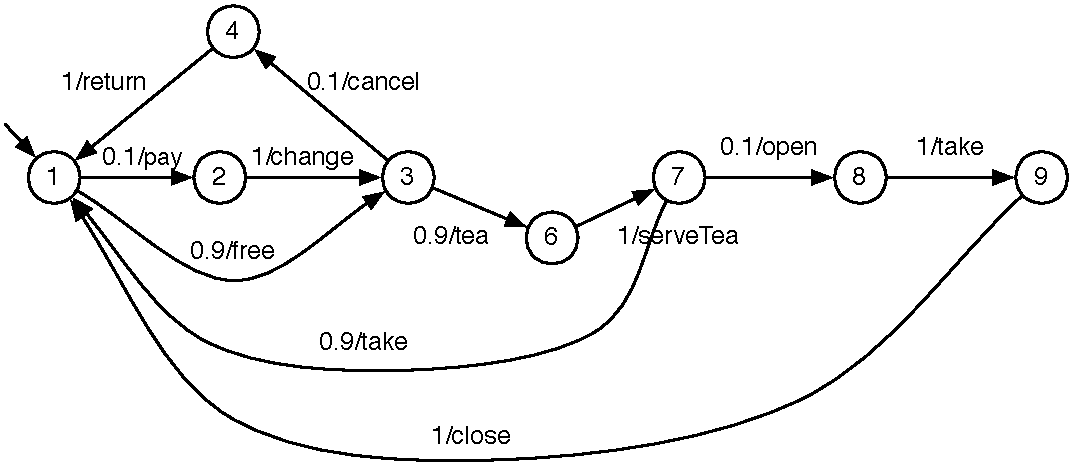
\includegraphics[width=95mm]{svm-usagemodel}
	\caption{Soda vending machine usage model}
	\label{fig:svmusagemodel}
\end{figure}

For instance, Figure \ref{fig:svmusagemodel} presents a usage model of the soda vending machine SPL described in section \ref{sec:casestudy:svm}: each transition has been tagged with a probability which represents, amongst all the possible products of the SPL, the probability of the transition to be fired. As we base our usage model on the actual usage of the product line, some states and transitions may be missing in the usage model if the behaviour linked to those states and transitions has not been observed in any product of the SPL. This corresponds to transitions with a probability equal to 0 and states with only input transitions with a probability equal to 0. In our example, we have no vending machine serving soda. Transitions with actions \textit{soda} and \textit{serve\-Soda} and state 5 have been removed from the usage model presented in Figure \ref{fig:svmusagemodel}.

The usage model is agnostic to the variability inherent to the SPL. It only represents the usage scenarios of the SPL under test as well as their respective probability and serves as basis to select test cases. There are two ways to associate usage scenarios to SPL products:  
%
\begin{itemize}
\item the \emph{family-based} approach \cite{Devroey2014,Devroey2015a} consists in exploiting logs as a source of user information and infer the usage model using machine learning techniques. We can then extract behaviour according to a probability range and relate them to the FTS and feature models of the SPL. As they are extracted from the usage model, behaviours can be run on the FTS to determine which products/features are involved. Some behaviours may also correspond to no product and thus no be executable. Those behaviours are errors coming from the usage model inference or indicators of errors in the FTS. Either case, they can be reported to the test engineer to correct the models.
%
\item the \emph{product-based} approach developed by Samih \etal \cite{Samih2014,Samih2014b} consists in creating usage models from the onset, taking into account requirements and feature models as well as translating expert knowledge to probabilities in the usage model. Concretely, requirements are related to features via a product matrix, while the usage model directly relates its transitions to probabilities and requirements of the SPL. Then, testers have to manually specify the products they are interested in and, with the help of the MaTeLo tool \cite{Samih2014c,matelo}, derive a pruned usage model corresponding  to the behaviour of these products and perform automated test case selection. 
\end{itemize}

%----------------------------------------
\subsection{Product-based test selection}
%----------------------------------------

Product-based test selection is straightforward: the test engineer selects one product to test by selecting features in the feature model, the tool then automatically use the projection operator on FTS to extract a LTS corresponding to the product, and prunes the usage model accordingly. The probabilities of the removed transitions are proportionally distributed on adjacent transitions, so that the probability axiom $\forall s_i \in S : \sum_{s_j \in S, \alpha_k \in \Act} P( s_i , \alpha_k, s_j ) = 1$ holds and balance between the probabilities of the transitions from a same source state are kept \cite{Samih2014b}. Finally, the tool selects test cases using statistical testing algorithms on the usage model~\cite{Whittaker1994,Feliachi2010}.

This scenario is proposed by Samih \etal \cite{Samih2014,Samih2014b} in the MaTeLo Product Line Manager (MPLM) tool \cite{Samih2014c}.  Product selection is made on an orthogonal variability model (OVM) and mapping between the OVM and the usage model (build by a system expert using MaTeLo \cite{matelo}) is provided via explicit traceability links to functional requirements. This process requires to perform the selection of the product of interest on the variability model and does not exploit the usage model during this selection. 


%----------------------------------------
\subsection{Family-based test selection}
%----------------------------------------

Contrary to product-based test selection, family-based test selection supports partial coverage of the SPL by the usage model (like the soda vending machine usage model presented in Figure \ref{fig:svmusagemodel}). 
The key idea is to select abstract test cases (\ie sequences of actions, not necessarily executable by one product of the SPL) from the usage model according to their probability to happen using an interval given by the engineer. Only abstract test cases from the model with a probability in this interval are considered. \Eg one may be interested in analysing highly probable behaviours (interval $[0.5 , 1]$). Only one abstract test case has a probability in this range in the soda vending machine usage model: $Pr(free, tea,serveTea,take) = 0.729$, which corresponds to the behaviour ``serving tea for free''.
The selected abstract test cases are filtered using the FTS in order to keep only positive abstract test cases (executable by at least one product of the SPL) and a pruned FTS (FTS'). The FTS' represents the minimal behaviour of the FTS needed to execute the positive abstract test cases, it is used latter to prioritize the products to test (see section \ref{sec:coverage:usage:prioritisation}).

\paragraph{Abstract test case selection from the usage model:}
%------------------------------------------------------------

The first step is to extract abstract test cases from the usage model according to the desired parameters. 
To perform abstract test case selection in a usage model $dtmc$, we apply an all-paths algorithm parametrized with a maximum length $l_{max}$ for finite abstract test cases and an interval $[Pr_{min} , Pr_{max}]$ specifying the minimal and maximal values for the probabilities of selected abstract test cases. 
Formally: 
\begin{align*}
    allpaths & (l_{max} , Pr_{min}, Pr_{max}, dtmc) =
        \{(i,\alpha_1 , ... , \alpha_{n}, i) \mid \\ 
        & n < lmax \wedge ( \nexists k : 0 < k < n, i = s_k ) \\
 \wedge &  (Pr_{min} \leq Pr(i,\alpha_1 , ... , \alpha_{n}, i) \leq Pr_{max})\}
\end{align*}
where 
$$Pr(i, \alpha_0, \dots, s_n) =\prod_{j=0}^{n-1} P_{dtmc}(s_j, \alpha_j , s_{j+1}).$$

We initially consider only (finite) abstract test cases starting from and ending in the initial state~$i$ (assimilated to an accepting state) without passing by~$i$ in between.  These abstract test cases correspond to a coherent execution scenario in the usage model. The $l_{max}$ bound allows the algorithm to scale to large usage models \cite{Devroey2014}.

The interval $[Pr_{min} , Pr_{max}]$ is provided by the engineer based on his knowledge of the SPL and the selection purpose: an interval with high values (\eg $[0.5 , 1]$) gives highly probable behaviours of the SPL. This is often desired for a non-regression testing scenario where the engineer wants to ensure that the main functionalities of a SPL are still  reliable after an update \cite{Mathur2008}. 
The engineer may also be interested in testing behaviours with a low probability as they may find rare bugs not discovered by the users of the products. Such strategies can be used, \eg for intrusion detection \cite{GarciaTeodoro2009}. 

The interval, its relevance, and selected test cases depend on the usage model source (\eg built from running products, manually built by an engineer, \etc) and the usage model shape (\ie number of states, transitions, average states degree, \etc). To have an idea of the interval to choose and the number of abstract test cases that are selected, the engineer may use random walks in the usage model to select random abstract test cases with their probability and see how they are distributed.

Practically, this algorithm builds an exploration tree where each node represents the exploration of a state. The exploration of a branch of the tree is stopped when the depth is higher than~$l_{max}$. This parameter is provided to the algorithm by the test engineer and is used to avoid infinite loops during the exploration of the usage model. 

For instance, the execution of the algorithm on the soda vending machine example ($um_{svm}$) presented in Figure \ref{fig:svmusagemodel}, with a $l_{max}$ value of 7 (the size of the maximal simple path) and an interval $[0, 0.1]$ to capture the least probable abstract test cases, gives 5 finite abstract test cases: 
\begin{align*}
& allpaths  (7 ;  0 ; 0.1 ; um_{svm}) = \{ \\ 
    & (pay, change, cancel, return) ; (free, cancel, return) ;\\
    & (pay, change, tea, serveTea, open, take,  close); \\
    & (pay, change, tea, serveTea, take) ; \\
    & (free, tea, serveTea, open, take, close)
    \}
\end{align*}
During the execution of the algorithm, the abstract test case \textit{(free, tea, serve\-Tea, take)} has been rejected since its probability ($0.729$) is not between $0$ and $0.1$.

The downside is that the algorithm may possibly enumerate all the paths in the usage model depending on the~$l_{max}$ value. This can be problematic and we plan in our future work to use symbolic executions techniques inspired by work in the probabilistic model checking area, especially automata-based representations \cite{Classen2011} in order to avoid exploring all paths.


\paragraph{FTS-based abstract test case filtering and FTS pruning:}
%-----------------------------------------------------------------

\begin{algorithm}[t]
	\KwIn{$\fts=(S,Act,\mathit{trans},i,d,\gamma)$: a connected FTS;\\
		  $s$: the set of abstract test cases to filter}
	\KwOut{$\fts'$, an FTS representing $\fts$ restricted to the behaviour in $s$, and $s'$, the set of positive abstract test cases from $s$}
	\Begin{
		$S' = \{i\}$; $\Act' = \emptyset$; $\trans'= \emptyset$; $i' = i$; $d' = d$; $\gamma' = \emptyset$\; \nllabel{algo:abstracttestcasesfiltering:line:init}
		$s' = s$\; \nllabel{algo:abstracttestcasesfiltering:line:init2}
		\For{$t \in \wTraces$ \nllabel{algo:abstracttestcasesfiltering:line:foreachtestcase}}{
			\eIf{$\exists s_k \in S,\: \fts \overset{t}{\Longrightarrow}s_k$ \nllabel{algo:abstracttestcasesfiltering:line:ifexecutable}}{
				$\Act' = \Act' \cup t$\; \nllabel{algo:abstracttestcasesfiltering:line:addaction}
				$S' = S' \cup \wStates(\fts, t)$\; \nllabel{algo:abstracttestcasesfiltering:line:addstates}
				$\trans' = \trans' \cup \wTransitions(\fts, t)$\; \nllabel{algo:abstracttestcasesfiltering:line:addtransitions}
				$\gamma' = \wFLabels(\fts, t) \gamma'$\; \nllabel{algo:abstracttestcasesfiltering:line:addfexpr}
			}{
				$s' = s' \setminus \{t\}$\; \nllabel{algo:abstracttestcasesfiltering:line:removetestcase}
			}
		}
		$\fts' = (S', \Act', \trans', i', d', \gamma')$\;
  		\Return $(\fts', s')$\; \nllabel{algo:abstracttestcasesfiltering:line:return}
	}
	\caption{FTS' building and positive abstract test cases filtering}
 \label{algo:abstracttestcasesfiltering}
\end{algorithm}

We do not make any assumptions about the source of the usage model. Therefore, this step serves as a sanity check to ensure that selected traces correspond to behaviour that may be executed by at least one valid product of the SPL. If this is not the case, there is an error in the usage model or in the FTS. 
Depending on how the model has been built, the error may come from the engineer (\eg missing transition/state, extra transition/state, wrong feature expression on a transition of the FTS, \etc during the modelling) or from the model inference method used to generate the model from a set of execution traces. Such errors have to be detected and reported to the engineer who has to decide what to do: either correct the usage model or the FTS in order to avoid illegal behaviours; or ignore the error if it is not significant.
 
The idea to filter abstract test cases and keep only positive abstract test cases is to use the FTS to detect negative abstract test cases by running them on it.
%
Practically, we build a second \emph{FTS} which represents only the behaviour of the SPL appearing in the positive abstract test cases selected from the usage model. This FTS' represents a prioritized subset of the original FTS \cite{Devroey2014e}.

Algorithm \ref{algo:abstracttestcasesfiltering} presents how to build the FTS' ($\fts'$) from a set of abstract test cases ($s$), with positive abstract test cases filtered during the algorithm (into $s'$), and a given FTS ($\fts$). 
The initial state of $fts'$ corresponds to the initial state of the $\fts$ (line \ref{algo:abstracttestcasesfiltering:line:init}) and $d$ in $\fts'$ is the same as for $\fts$ (line \ref{algo:abstracttestcasesfiltering:line:init}). 
For each abstract test case, if it is executable on $\fts$ (line \ref{algo:abstracttestcasesfiltering:line:ifexecutable}), then the states ($states(fts, t)$), actions ($t$) and transitions ($\wTransitions(fts, t)$) visited in $\fts$ when executing the trace $t$ are added to $\fts'$ (line \ref{algo:abstracttestcasesfiltering:line:addaction} to \ref{algo:abstracttestcasesfiltering:line:addtransitions}). 
%
On line~\ref{algo:abstracttestcasesfiltering:line:addfexpr}, the $\wFLabels(\fts, t)$ function is used to enrich the $\gamma'$ function with the feature expressions of the transitions visited when executing $t$ on the $\fts$. It has the following signature: 
%
$$\wFLabels : (\FTS, \Act^{*}) \rightarrow (\trans \mapsto \Sem{d} \mapsto \mathbb{B}) \rightarrow (\trans \mapsto \Sem{d} \mapsto \mathbb{B})$$
%
On line \ref{algo:abstracttestcasesfiltering:line:addfexpr}, $\wFLabels (\fts, t) \gamma_{\fts'}$ returns a new function $\gamma'_{\fts'}$ which, for a given transition $tr = (s_i \overset{\alpha_k}{\longrightarrow}  s_{j}) $, returns $\gamma_{\fts} (tr)$ if $\alpha_k \in t$ or $\gamma_{\fts'} (tr)$ otherwise.

\begin{figure}
	\centering
	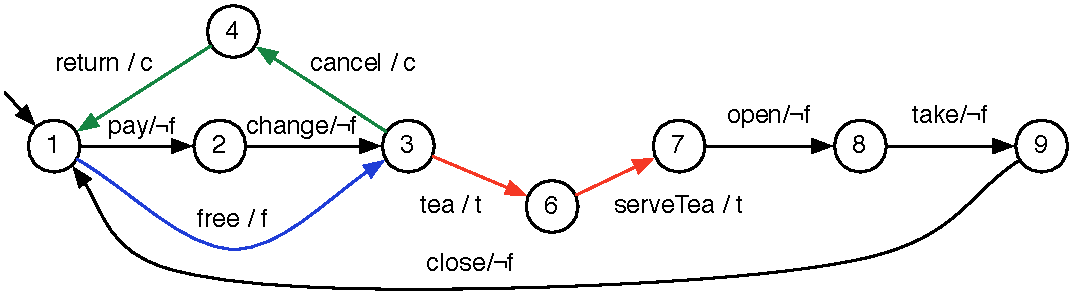
\includegraphics[width=95mm]{svm-ftsprime}
	\caption{Soda vending machine FTS'}
	\label{fig:svmftsprime}
\end{figure}

In our example, the set of finite traces with a probability between 0 and 0.1 selected in step~1 contains two negative abstract test cases: \textit{(pay, change, tea, serve\-Tea, take)} and \textit{(free, tea, serve\-Tea, open, take, close)}, which both lead to an execution condition containing the $free \wedge \neg free$ feature expression. Those 2 negative abstract test cases (mixing free and not free vending machines) cannot be executed on the soda vending machine  FTS (of Figure \ref{fig:svmfts}) and are rejected by Algorithm \ref{algo:abstracttestcasesfiltering}. The generated FTS' is presented in Figure \ref{fig:svmftsprime}.

%-----------------------------------
\subsection{Product prioritisation}
%-----------------------------------

\label{sec:coverage:usage:prioritisation}

Product-based test selection assumes that relevant products from which test cases are selected have already been prioritized. Relevant products are used to prune the usage model (in order to keep only the behaviour of the selected product) and test cases are derived using a statistical testing algorithm.

When performing a family-based test selection from a usage model, relevant abstract test cases are directly selected from the usage model representing the behaviour of the SPL. Those abstract test cases are then filtered to keep only positive abstract test cases. At the end of algorithm \ref{algo:abstracttestcasesfiltering}, we have an FTS' and a set of (positive abstract) test cases. This set of test cases covers all states and transitions of the FTS'. Since they come from the usage model, it is possible to order them according to their probability to happen. This probability corresponds to the the cumulated individual probabilities of the transitions fired when executing the finite trace in the usage model. 
A test case $t=(i, \alpha_1 , \ldots , \alpha_n, i)$ corresponding to a path $(i \overset{\alpha_1}{\longrightarrow} \ldots \overset{\alpha_n}{\longrightarrow} i)$ in the usage model has a probability $\wPr(i, \alpha_1 , \ldots , \alpha_n, i)$ to be executed. 

At this step, each test case $t$ is associated to the set of products $\wProd(t,\fts')$ that can actually execute~$t$. Product prioritisation may be done by sorting the test cases according to their probability to be executed, giving a set of products for each test case $t$.

For instance, for the positive abstract test case $t = $ \textit{(pay, change, tea, serve\-Tea, open, take, close)}, selected for our example, the products have to satisfy: $$\neg f \wedge t \wedge \CNF(d)$$
Where $d$ is the feature model of the soda vending machine (presented in Figure \ref{fig:svmfm}), transformed into a boolean formula using the $\CNF$ function.
This gives us a set of 8 products (amongst 32 possible):
\begin{align*}
\{&(v, b, cur, t, eur) ; (v, b, cur, t, usd) ; (v, b, cur, t, c, eur) ; \\
& (v, b, cur, t, c, usd) ; (v, b, cur, t, s, eur) ; (v, b, cur, t, s, usd) ;\\
&(v, b, cur, t, s, c, eur) ; (v, b, cur, t, s, c, usd) \}
\end{align*}
Each of them executing $t$, which is the behaviour of the soda vending machine product line with the lowest probability ($\wPr(t) = 0.009$ in the usage model). 

%-------------------------
\subsection{Related work}
%-------------------------

To the best of our knowledge, there is no approach prioritizing behaviours statistically for testing SPLs in a family-based manner.  
There have been SPL test efforts to sample products for testing such as t-wise approaches \cite{Perrouin2011,Cohen2006,Cohen2008,Johansen2012}. More recently sampling was combined with prioritisation thanks to the addition of weights on feature models and the definition of multiple objectives \cite{Johansen2012b,Henard2014a}. However, these approaches do not consider SPL behaviour in their analyses.  

Efforts to combine sampling techniques with modelling ones (\eg \cite{Lochau2011}) exist.  These approaches are product-based, meaning that they may miss opportunities to reuse tests amongst sampled products \cite{VonRhein2013}. We believe that benefiting from the recent advances in behavioural modelling provided by the model checking community \cite{Asirelli2011,Asirelli2011a,Classen2011,Classen2013b,Fischbein2006,Lauenroth2009,Rodrigues2015,terBeek2016}, sound MBT approaches for SPL can be derived and interesting scenarios combining verification and testing can be devised.

To consider behaviour in an abstract way, a full-fledged MBT approach \cite{Utting2007} is required. Although behavioural MBT is well established for single-system testing~\cite{Tretmans2008}, a survey  \cite{Oster2011} shows insufficient support for SPL-based MBT. Metzger and Pohl further emphasizes the need for inter-model consistency  and minimizing test redundancy  across the lifecycle (domain and application engineering) \cite{Metzger2014}. We believe that the FTS formalism, natively equipped with features as a first-class concept, is pivotal  to inter-model verification support and supports combination of quality assurance techniques both at the domain and application engineering levels as our integration between family-based and product-based statistical test selection illustrates.  

Our will is to apply ideas stemming from statistical testing \cite{Sprenkle2013} and adapt them in an SPL context. For example, combining structural criteria with statistical testing has been discussed by Gouraud \etal  \cite{Gouraud2001} and Th\'evenod-Fosse and Waeselynck \cite{Thevenod-Fosse1991}. We do not make any assumption on the way the usage model is obtained: via an operational profile \cite{Musa1996}, by analysing the source code or the specification \cite{Thevenod-Fosse1991}, or from the running application logs \cite{Ghezzi2014,Sprenkle2013}. In the absence of a source of information for the usage model, one could think of a uniform distribution of probabilities over the usage model. As noted by Whittaker \cite{Whittaker1994}, in such case, only the structure of abstract test cases would be considered and therefore basing their selection on their probabilities would just be a means to limit their number in a mainly random testing approach. In such cases, it is better to use structural test selection  \cite{Feliachi2010}.

We use MaTeLo \cite{matelo} to select test cases from a product model. Other tools like JUMBL \cite{Prowell2003} would have qualified. Both are model-based statistical testing tools, supporting the development of statistical usage models using Markov chains, the analysis of models, and the selection of test cases \cite{Utting2012}. However, none of them are able to natively handle SPL models. We use the MaTeLo Product Line Manager (MPLM) tool \cite{Samih2014,Samih2014b} to generate models for a product of the SPL, which are then used to select test cases. 


%%%%%%%%%%%%%%%%%%%%%%%%%%%%%%%%%%%%
\section{Wrap up}
%%%%%%%%%%%%%%%%%%%%%%%%%%%%%%%%%%%%

In this chapter, we described three abstract test case selection and prioritisation approaches: structural, dissimilarity, and usage based test cases selection criteria. 

\paragraph{Structural selection criteria:}
%--------------------------------------------

Structural selection and prioritisation criteria are based on the structure of the \gls{FTS} representing the product line to test. Those criteria consider the number of states, actions, transitions, transitions-pairs, or paths covered in the FTS to guide the abstract test case selection. Once selected, the prioritisation of the products to test is done according to the abstract test cases executable by those products: products that can reach the best coverage by executing as many test cases as possible and/or those with the best coverage are ranked first. 

\paragraph{Dissimilarity selection criteria:}
%--------------------------------------------

Dissimilarity selection criteria aim at selecting abstract test cases as diverse as possible. The dissimilarity is defined by the test engineer by combining basic distance functions taking the actions and products covered by the test cases as input. We used a (1+1) without mutation nor crossover evolutionary algorithm to select the test cases, based on a given time budget and a given size of the test suite.

\paragraph{Usage selection criteria:}
%--------------------------------------------

Usage-based selection criteria may be used in two ways: family-based and product-based test selection and prioritisation. Family-based selection and prioritisation extracts products of interest according to the probability of their execution traces gathered in a usage model.  We thus select a subset of the full SPL behaviour given as a \gls{FTS}. This allows us to construct a new FTS, FTS', representing only the executions of relevant products.  This FTS' can be analysed all at once to enable test reuse amongst products to scale during testing activities. Product-based selection and prioritisation requires the testers to select a product of interest before the usage model is pruned, leaving only its executions associated to it \cite{Samih2014b,Samih2014,Samih2014c}. Though these approaches may seem antagonistic, family-based prioritisation can gracefully complement the product-based one by suggesting products of interest.
